\qns{Capacitor with a Periodic Current Source}

\textbf{Learning Goal:} This problem aims to make students familiar with the charging/ discharging response of a capacitor.

\textbf{Relevant Notes:} \notes{Note 17} covers capacitive behavior in the presence of difference types of current sources.

Capacitive touchscreen requires detection of capacitance change due to touch. If we connect a known current source $I_s$ to the capacitor and
measure the voltage across the capacitor $V$, we will be able to solve for the capacitance $C$. So we build the following circuit to measure with a periodic current source:
\begin{center}
	\begin{circuitikz}[american voltages, american currents] 
		\draw (0, 0) to [I, l=$I_s(t)$] (0, 4) -- (2, 4) to [C=$C$] (2, 0) -- (0, 0);
		\draw (0, 0) to [short, -o] (6, 0);     
		\draw (2, 4) to [short, -o] (6, 4);
		\draw (6, 3.8) to [open, v= $V(t)$](6, 0.2);
		\draw (-3, 1.7) to (-2.6, 1.7) to (-2.6, 2.3) to (-2.2, 2.3) to (-2.2, 1.7) to (-1.8, 1.7) to (-1.8, 2.3) to (-1.4, 2.3);
	\end{circuitikz}
\end{center}

\meta{
When explaining the relationship between current and voltage, it might be helpful to explain how the current is proportional to the change in voltage over time ($I = C\frac{dV}{dt}$). Even though calculus isn’t really emphasized much in the class, some students may find it helpful to see how the voltage signal is the integral of the current signal, so the slope of the voltage depends on the value of the current within a given interval.

For the time intervals ($\frac{T}{2}$, $T$, etc.) there's no significant difference between $<$ and $\leq$ because the function $V(t)$ is continuous.
}

\begin{enumerate}
\item
Let us assume the current $I_s$ is a function of time as follows:

\begin{center}
	\begin{tikzpicture}
	\begin{axis}[
	xmin=-5, xmax=60,
	ymin=-160, ymax=160,
	axis lines=center,
	axis on top=true,
	grid style={dashed},
	xlabel={\emph{$t$}},
	ylabel={\emph{$I_s(t)$}},
	yticklabels={,,},
	xticklabels={,,},
	width=6in,
	height=3in,
	]
	\addplot [draw=red,thick] coordinates {(0, 0) 
		(0, 100) (10, 100)
		(10, -100) (20, -100)
		(20, 100) (30, 100)
		(30, -100) (40, -100)
		(40, 100) (50, 100)
		(50, -100) (60, -100)};
	\node [left,color=red] at (axis cs:  0, 100) {$I_1$}; 
	\node [left,color=red] at (axis cs:  0, -100) {$-I_1$}; 
	\node [below,color=red] at (axis cs:  19, 0) {$T$};
	\node [below,color=red] at (axis cs:  9, 0) {$\frac{T}{2}$};
	\node [below,color=red] at (axis cs:  39, 0) {$2T$}; 
	\node [below,color=red] at (axis cs:  29, 0) {$\frac{3T}{2}$};
	\end{axis}
	\end{tikzpicture}
\end{center}

What does the voltage $V$ look like with this current source? Let's assume that the capacitor is initially uncharged (i.e. $Q = 0$). Since $Q=CV$, this means that at time $t=0$ the voltage $V=0$. 

\ans{
When a constant current source is applied to a capacitor, we know that the voltage obeys the following equation
\begin{align} \label{eq:cap_voltage}
V_C(t) = \frac{I}{C} t + V_C(0).
\end{align}
Our periodic current source $I_s$ is constant from $t=0$ to $t=\frac{T}{2}$, so we can apply equation \ref{eq:cap_voltage} over this time period. We know the initial voltage is zero, so:
\begin{align*}
V(t) = \frac{I_1}{C}t \quad \text{when } 0\leq t \leq \frac{T}{2}
\end{align*}

\begin{center}
	\begin{tikzpicture}
	\begin{axis}[
	xmin=-5, xmax=60,
	ymin=-160, ymax=160,
	axis lines=center,
	axis on top=true,
	grid style={dashed},
	xlabel={\emph{$t$}},
	ylabel={\color{red}{\emph{$I_s(t)$}}},
	yticklabels={,,},
	xticklabels={,,},
	width=6in,
	height=3in,
	]
	\addplot [draw=red,thick] coordinates {(0, 0) 
		(0, 100) (10, 100)
		(10, -100) (20, -100)
		(20, 100) (30, 100)
		(30, -100) (40, -100)
		(40, 100) (50, 100)
		(50, -100) (60, -100)};
	\node [left,color=red] at (axis cs:  0, 100) {$I_1$}; 
	\node [left,color=red] at (axis cs:  0, -100) {$-I_1$}; 
	\node [below,color=red] at (axis cs:  19, 0) {$T$};
	\node [below,color=red] at (axis cs:  9, 0) {$\frac{T}{2}$};
	\node [below,color=red] at (axis cs:  39, 0) {$2T$}; 
	\node [below,color=red] at (axis cs:  29, 0) {$\frac{3T}{2}$};
	% voltage
	\node[left, color=blue] at (axis cs: 0, 145) {$V(t)$};
	\addplot [draw=blue,thick] coordinates{ (0,0) (10, 45)};
	\node [above, color=blue] at (axis cs: 2, 25) {slope = $\frac{I_1}{C}$};
	%\node [above, color=blue] at (axis cs: 10,50) {$V = \frac{IT}{2C}$};
	\end{axis}
	\end{tikzpicture}
\end{center}

In order to figure out what happens next, let's consider a more generic version of equation \ref{eq:cap_voltage}:
\begin{align} \label{eq:cap_voltage2}
V_C(t) = \frac{I}{C} (t-t_0) + V_C(t_0).
\end{align}
With this equation, we can consider an arbitrary starting time $t_0$ instead of always starting at $t=0$. Plugging in $t_0=0$ yields equation \ref{eq:cap_voltage}. Like equation \ref{eq:cap_voltage}, the above equation is only true when the current is constant.

The next time period with constant current is from $t=\frac{T}{2}$ to $t=T$. Over this time, the current through the capacitor is $-I_1$. Since we are starting at time $\frac{T}{2}$, we set $t_0 = \frac{T}{2}$ and plug into equation \ref{eq:cap_voltage2}.
\begin{align*}
V(t) &= \frac{-I_1}{C}\left(t-\frac{T}{2}\right) + V\left(\frac{T}{2}\right) \\
V(t) &= \frac{-I_1}{C}\left(t-\frac{T}{2}\right) + \frac{I_1 T}{2C} \\
\end{align*}

Combining with our previous relationship yields:

\begin{equation*} 
V_C(t) = 
\begin{cases}
	\frac{I_1}{C}t & \text{when } 0\leq t \leq \frac{T}{2} \\
	\frac{-I_1}{C}\left(t-\frac{T}{2}\right) + \frac{I_1 T}{2C}
	&
	\text{when }  \frac{T}{2} < t \leq T
\end{cases}
\end{equation*}
\begin{center}
	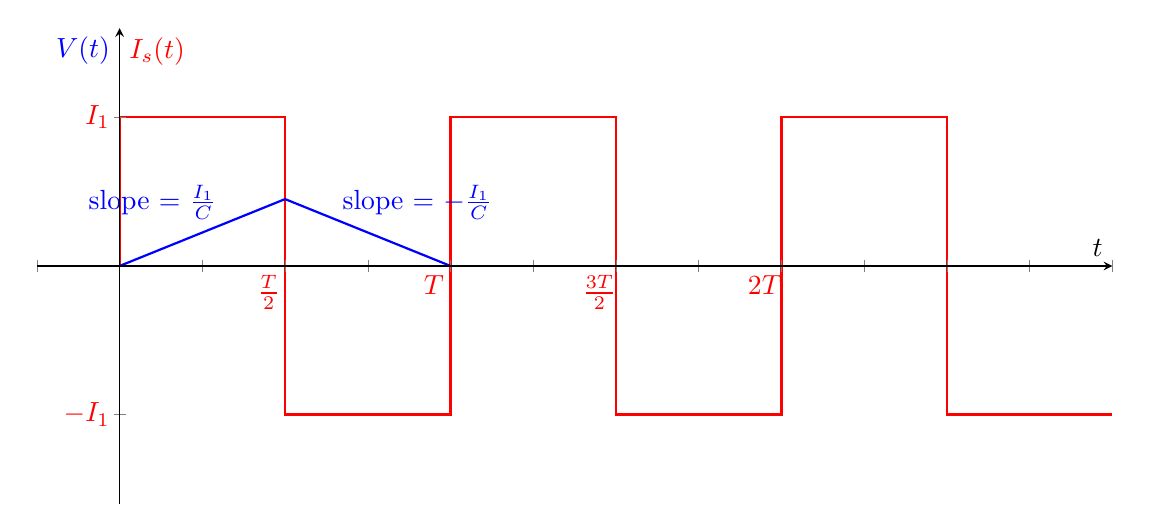
\begin{tikzpicture}
	\begin{axis}[
	xmin=-5, xmax=60,
	ymin=-160, ymax=160,
	axis lines=center,
	axis on top=true,
	grid style={dashed},
	xlabel={\emph{$t$}},
	ylabel={\color{red}{\emph{$I_s(t)$}}},
	yticklabels={,,},
	xticklabels={,,},
	width=6in,
	height=3in,
	]
	\addplot [draw=red,thick] coordinates {(0, 0) 
		(0, 100) (10, 100)
		(10, -100) (20, -100)
		(20, 100) (30, 100)
		(30, -100) (40, -100)
		(40, 100) (50, 100)
		(50, -100) (60, -100)};
	\node [left,color=red] at (axis cs:  0, 100) {$I_1$}; 
	\node [left,color=red] at (axis cs:  0, -100) {$-I_1$}; 
	\node [below,color=red] at (axis cs:  19, 0) {$T$};
	\node [below,color=red] at (axis cs:  9, 0) {$\frac{T}{2}$};
	\node [below,color=red] at (axis cs:  39, 0) {$2T$}; 
	\node [below,color=red] at (axis cs:  29, 0) {$\frac{3T}{2}$};
	% voltage
	\node[left, color=blue] at (axis cs: 0, 145) {$V(t)$};
	\addplot [draw=blue,thick] coordinates{ (0,0) (10, 45) (20, 0)};
	\node [above, color=blue] at (axis cs: 2, 25) {slope = $\frac{I_1}{C}$};
	\node [above, color=blue] at (axis cs: 18, 25) {slope = $-\frac{I_1}{C}$};
	%\node [above, color=blue] at (axis cs: 10,50) {$V = \frac{IT}{2C}$};
	\end{axis}
	\end{tikzpicture}
\end{center}

To determine the full behavior of $V(t)$, we could continue to apply equation \ref{eq:cap_voltage2} for each period of constant current. However, we notice that at $t=T$, the voltage and current are the same as they were at $t=0$. Since the current source is periodic (repeats every $T$), the voltage pattern will also repeat. 

\begin{center}
	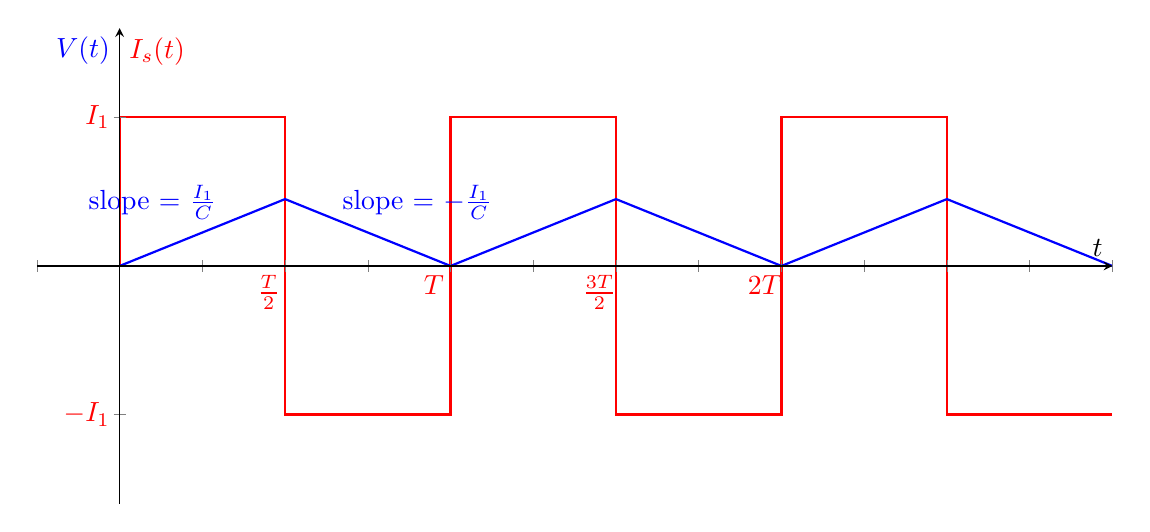
\begin{tikzpicture}
	\begin{axis}[
	xmin=-5, xmax=60,
	ymin=-160, ymax=160,
	axis lines=center,
	axis on top=true,
	grid style={dashed},
	xlabel={\emph{$t$}},
	ylabel={\color{red}{\emph{$I_s(t)$}}},
	yticklabels={,,},
	xticklabels={,,},
	width=6in,
	height=3in,
	]
	\addplot [draw=red,thick] coordinates {(0, 0) 
		(0, 100) (10, 100)
		(10, -100) (20, -100)
		(20, 100) (30, 100)
		(30, -100) (40, -100)
		(40, 100) (50, 100)
		(50, -100) (60, -100)};
	\node [left,color=red] at (axis cs:  0, 100) {$I_1$}; 
	\node [left,color=red] at (axis cs:  0, -100) {$-I_1$}; 
	\node [below,color=red] at (axis cs:  19, 0) {$T$};
	\node [below,color=red] at (axis cs:  9, 0) {$\frac{T}{2}$};
	\node [below,color=red] at (axis cs:  39, 0) {$2T$}; 
	\node [below,color=red] at (axis cs:  29, 0) {$\frac{3T}{2}$};
	% voltage
	\node[left, color=blue] at (axis cs: 0, 145) {$V(t)$};
	\addplot [draw=blue,thick] coordinates{ (0,0) (10, 45) (20, 0)(30, 45)(40, 0)(50, 45)(60, 0)};
	\node [above, color=blue] at (axis cs: 2, 25) {slope = $\frac{I_1}{C}$};
	\node [above, color=blue] at (axis cs: 18, 25) {slope = $-\frac{I_1}{C}$};
	%\node [above, color=blue] at (axis cs: 10,50) {$V = \frac{IT}{2C}$};
	\end{axis}
	\end{tikzpicture}
\end{center}
}

\item
Now let us assume the current $I_s$ is a function of time as follows:

\begin{center}
	\begin{tikzpicture}
	\begin{axis}[
	xmin=-5, xmax=60,
	ymin=-160, ymax=160,
	axis lines=center,
	axis on top=true,
	grid style={dashed},
	xlabel={\emph{$t$}},
	ylabel={\emph{$I_s(t)$}},
	yticklabels={,,},
	xticklabels={,,},
	width=6in,
	height=3in,
	]
	\addplot [draw=red,thick] coordinates {(0, 0) 
		(0, 100) (10, 100)
		(10, 0) (20, 0)
		(20, 100) (30, 100)
		(30, 0) (40, 0)
		(40, 100) (50, 100)
		(50, 0) (60, 0)};
	\node [left,color=red] at (axis cs:  0, 100) {$I_1$}; 
	\node [left,color=red] at (axis cs:  0, -100) {$-I_1$}; 
	\node [below,color=red] at (axis cs:  19, 0) {$T$};
	\node [below,color=red] at (axis cs:  9, 0) {$\frac{T}{2}$};
	\node [below,color=red] at (axis cs:  39, 0) {$2T$}; 
	\node [below,color=red] at (axis cs:  29, 0) {$\frac{3T}{2}$};
	\end{axis}
	\end{tikzpicture}
\end{center}

What does the voltage $V$ qualitatively look like with this current source? Draw out on the above graph how the voltage changes over time, starting at time $t = 0$. Let's assume that the capacitor is initially uncharged (i.e. $Q = 0$). Since $Q=CV$, this means that at time $t=0$ the voltage $V=0$. 

\meta {Even though the current source signal returns to zero, the given voltage across the capacitor doesn’t go to zero until the capacitor is discharged, or disconnected from the current source.}

\ans{

In the first segment, when $0 \leq t \leq \frac{T}{2}$, we found in part (a) using equation \ref{eq:cap_voltage2} that $$V_C(t) = \frac{I}{C} t$$
However, when $\frac{T}{2} < t \leq T$, $I_s(t)$ is now 0. 
We again use equation \ref{eq:cap_voltage2} from part (a)
\begin{align*}
V_C(t) = \frac{I}{C} (t-t_0) + V_C(t_0).
\end{align*}
knowing that $t_0 = \frac{T}{2}$. To find $V_C(t_0)$, we can use the fact that $0 \leq t \leq \frac{T}{2}$ when $t = t_0$ to get $V_c(t_0) = \frac{I_1}{C} \frac{T}{2}$. Plugging these values into equation \ref{eq:cap_voltage2} gives:
$$V_C(t) = \frac{0}{C} (t-\frac{T}{2}) + \frac{I_1}{C} \frac{T}{2} = \frac{I_1 T}{2C}$$
Qualitatively, this indicates that $V_C(t)$ is held constant whenever $I_s(t) = 0$. However, when $I_s(t) = I_1$, $V_C(t)$ goes upwards with slope $\frac{I_1}{C}$, starting from the constant value of $V_C(t)$ while its slope is 0.
\begin{center}
	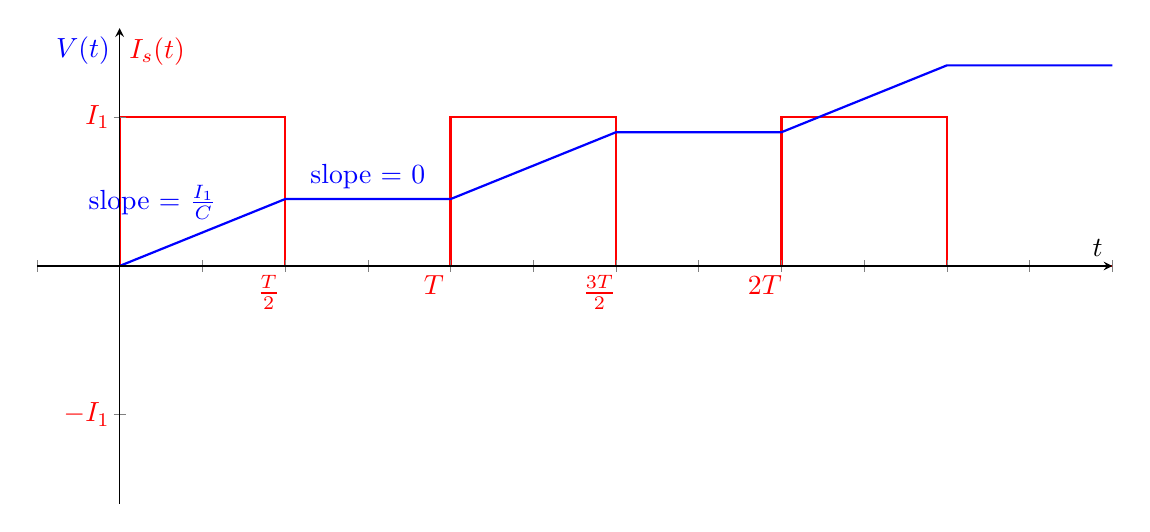
\begin{tikzpicture}
	\begin{axis}[
	xmin=-5, xmax=60,
	ymin=-160, ymax=160,
	axis lines=center,
	axis on top=true,
	grid style={dashed},
	xlabel={\emph{$t$}},
	ylabel={\color{red}{\emph{$I_s(t)$}}},
	yticklabels={,,},
	xticklabels={,,},
	width=6in,
	height=3in,
	]
	\addplot [draw=red,thick] coordinates {(0, 0) 
		(0, 100) (10, 100)
		(10, 0) (20, 0)
		(20, 100) (30, 100)
		(30, 0) (40, 0)
		(40, 100) (50, 100)
		(50, 0) (60, 0)};
	\node [left,color=red] at (axis cs:  0, 100) {$I_1$}; 
	\node [left,color=red] at (axis cs:  0, -100) {$-I_1$}; 
	\node [below,color=red] at (axis cs:  19, 0) {$T$};
	\node [below,color=red] at (axis cs:  9, 0) {$\frac{T}{2}$};
	\node [below,color=red] at (axis cs:  39, 0) {$2T$}; 
	\node [below,color=red] at (axis cs:  29, 0) {$\frac{3T}{2}$};
	% voltage
	\node[left, color=blue] at (axis cs: 0, 145) {$V(t)$};
	\addplot [draw=blue,thick] coordinates{ (0,0) (10, 45) (20, 45)(30, 90)(40, 90)(50, 135)(60, 135)};
	\node [above, color=blue] at (axis cs: 2, 25) {slope = $\frac{I_1}{C}$};
	\node [above, color=blue] at (axis cs: 15, 45) {slope = $0$};
	%\node [above, color=blue] at (axis cs: 10,50) {$V = \frac{IT}{2C}$};
	\end{axis}
	\end{tikzpicture}
\end{center}
}
\end{enumerate}